\chapter{\ifproject%
\ifenglish Project Structure and Methodology\else โครงสร้างและขั้นตอนการทำงาน\fi
\else%
\ifenglish Project Structure\else โครงสร้างของโครงงาน\fi
\fi
}

% ในบทนี้จะกล่าวถึงหลักการ และการออกแบบระบบ

\makeatletter

% \renewcommand\section{\@startsection {section}{1}{\z@}%
%                                    {13.5ex \@plus -1ex \@minus -.2ex}%
%                                    {2.3ex \@plus.2ex}%
%                                    {\normalfont\large\bfseries}}

\makeatother
%\vspace{2ex}
% \titleformat{\section}{\normalfont\bfseries}{\thesection}{1em}{}
% \titlespacing*{\section}{0pt}{10ex}{0pt}

\section{Methodology}

\subsection{System Architecture}
 The proposed framework consists of two ESP32 devices, each connected to a LoRa SX1276 module. One device operates as the sender (initiator), and the other as the receiver (responder). The devices communicate over LoRa to exchange verification and application messages. The overall architecture ensures that both devices can generate identical session keys without directly transmitting key material.

\begin{figure}[htbp]
\begin{center}
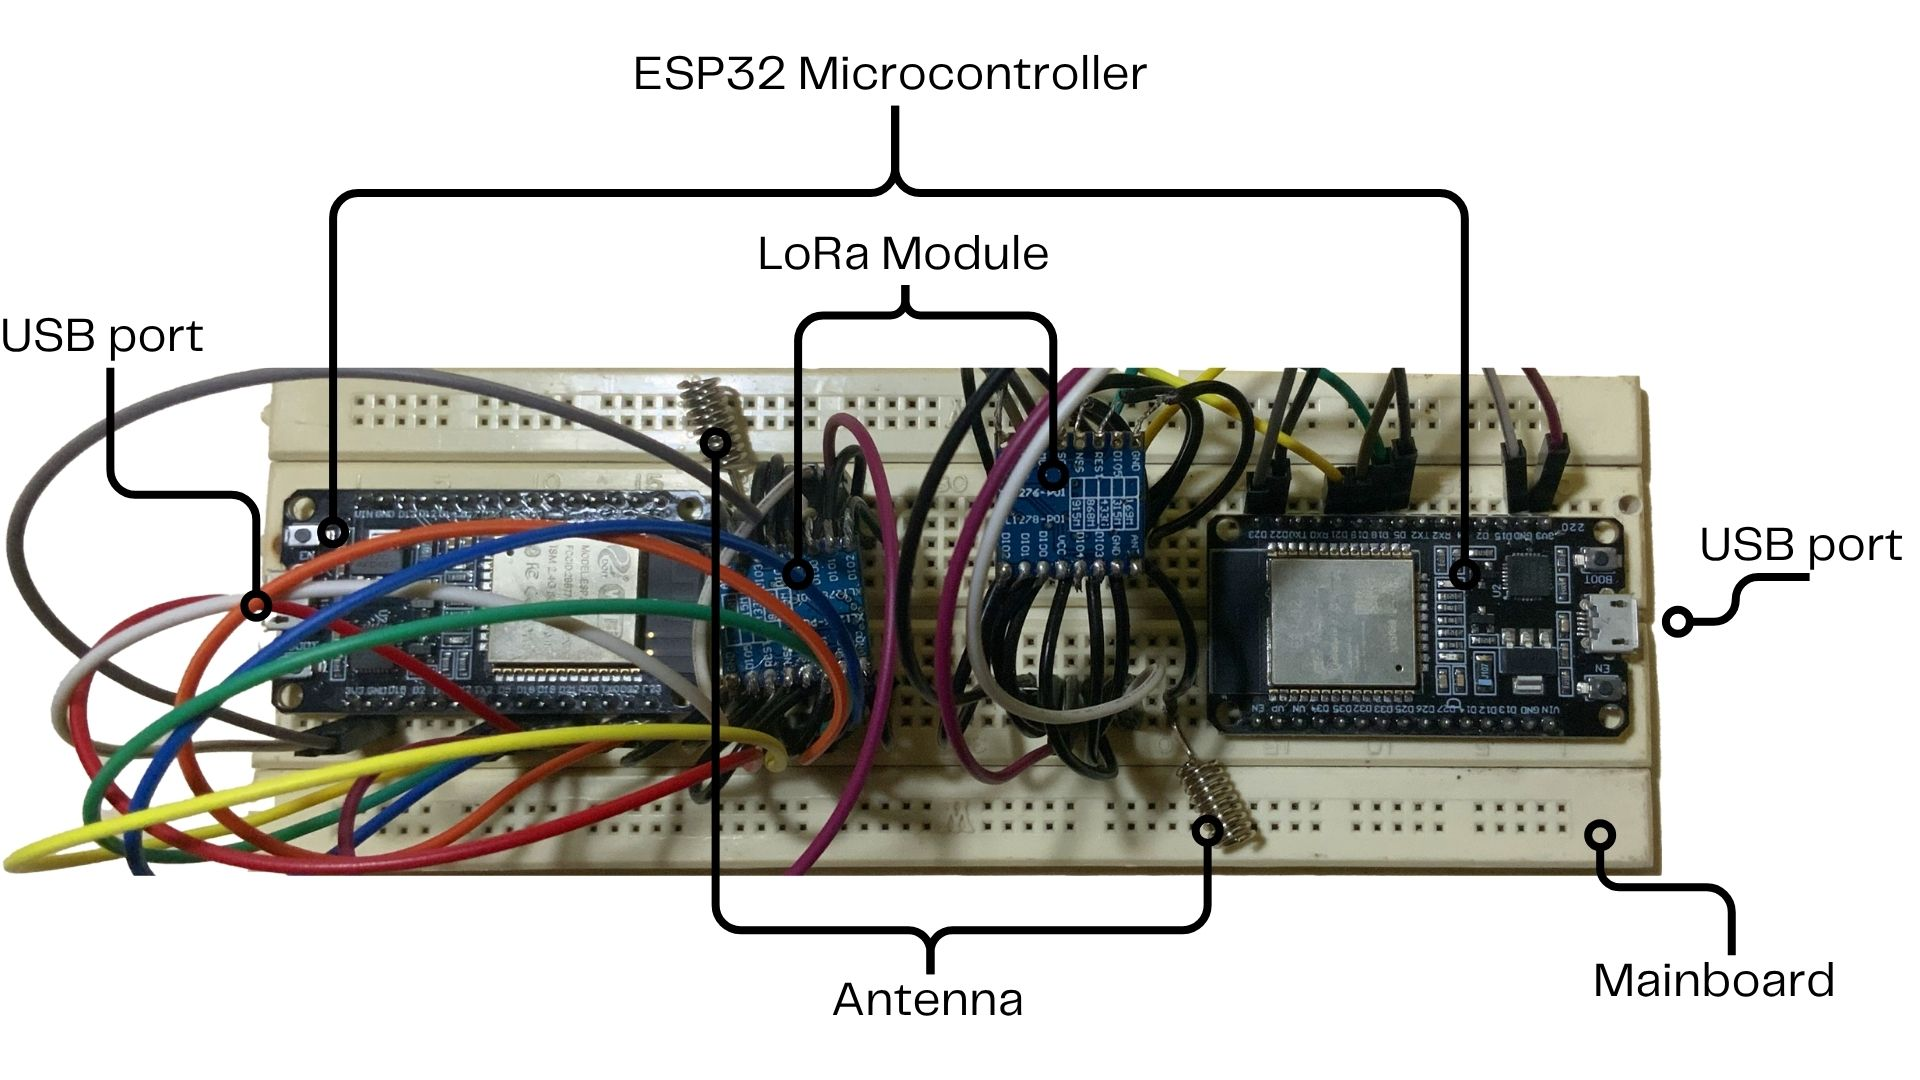
\includegraphics[width=0.8\textwidth]{Architecture.jpg}
\end{center}
\caption[Picture]{Design Architecture}
\label{fig:architecture}
\end{figure}

\subsection{RSSI-Based Key Generation}
To synchronize RSSI values, one device (the initiator) first transmits a known verification message. The receiving device measures the RSSI of this signal and attempts to decode the message using its reading. If decryption fails, the receiver iteratively adjusts its interpretation by shifting the RSSI value up or down within a pre-agreed tolerance interval (e.g., ±0.5 dBm) until the message is correctly decrypted. Unlike static pre-shared keys, which remain fixed and are vulnerable once compromised, session keys in this framework are dynamically derived from RSSI. Since RSSI is measured uniquely at the receiver and varies naturally with the environment, it is difficult for an attacker to predict or replicate. Security is further enhanced by concatenating the RSSI values and sampling them across multiple frequency channels into an array. 

\subsection{Keyword Verification}
To ensure correctness, both devices share a pre-defined keyword. After decryption, the receiver compares the result against this keyword. A match confirms that both devices are synchronized on the same session key. If the keyword is not matched, the process repeats until a valid session key is established.

\subsection{System Implementation}

\subsubsection{Hardware Setup}
The following components are required for the system implementation:
\begin{itemize}
    \item ESP32 development board (MicroPython-compatible)
    \item SX1276 LoRa module
    \item USB cable for ESP32
    \item Jumper wires
    \item Computer with \texttt{esptool.py} and \texttt{mpremote} installed
\end{itemize}

\subsubsection{Pin Mapping}
The interfacing between the ESP32 and the SX1276 module is established through the SPI bus and control lines.  
The pin assignments are listed in Table~\ref{tab:pinmapping}. These may be modified in \texttt{lora.py} as required.

\begin{table}[htbp]
\centering
\label{tab:pinmapping}
\begin{tabular}{|c|c|}
\hline
\textbf{Signal} & \textbf{ESP32 GPIO Pin} \\ \hline
MISO & GPIO19 \\ \hline
MOSI & GPIO23 \\ \hline
SCK  & GPIO18 \\ \hline
CS   & GPIO5  \\ \hline
RST  & GPIO17 \\ \hline
DIO0 & GPIO26 \\ \hline
\end{tabular}
\caption{Pin Mapping between ESP32 and LoRa Module}
\end{table}

\subsection{Flashing MicroPython on ESP32}

To run the ESP32 with MicroPython, follow these steps:

\subsubsection{Erase Existing Flash}
Before flashing, erase the current firmware on the ESP32:

\begin{verbatim}
esptool --port COM6 erase_flash
\end{verbatim}

\noindent This clears the flash memory of a standard ESP32.

\subsubsection{Write MicroPython Firmware}
Next, write the MicroPython firmware to the ESP32. Replace {<micropython-firmware.bin>} with your firmware file name:

\begin{verbatim}
esptool --baud 460800 write_flash 0 \
ESP32_GENERIC_C6-20250415-v1.25.0.bin
\end{verbatim}


\noindent Example using a specific firmware file:

\begin{verbatim}
esptool --baud 460800 write_flash 0 ESP32_GENERIC_C6-20250415-v1.25.0.bin
\end{verbatim}

\noindent After flashing, the ESP32 is ready to run MicroPython scripts via a serial connection.

\subsection{Prepare and Upload Files}

Before running the system, edit the \texttt{lora.py} file locally to ensure the pin mapping matches your ESP32 configuration (see Section~\ref{tab:pinmapping}).

\subsubsection{Upload \texttt{lora.py} to ESP32}
Use \texttt{mpremote} to upload the Python script to the ESP32:

\begin{verbatim}
mpremote connect COM6 fs cp lora.py 
\end{verbatim}

\noindent Explanation:
\begin{itemize}
    \item \texttt{mpremote connect COM6} — Connects to the ESP32 on port COM6.
    \item \texttt{fs cp lora.py :} — Copies the \texttt{lora.py} file to the root directory of the ESP32 filesystem.
\end{itemize}

After uploading, the ESP32 is ready to run the LoRa communication program.

\subsection{Connect to Shell and Run}

After uploading the necessary files, follow these steps to execute the program on the ESP32 nodes.

\begin{enumerate}
    \item Connect the ESP32 to your computer via USB.
    
    \item Open the serial REPL using \texttt{mpremote}:

\begin{verbatim}
mpremote connect /dev/ttyUSB0 repl
\end{verbatim}
    
    \item Upload and run the application scripts:
    \begin{itemize}
        \item On Node A (sender): upload and run \texttt{sender.py}.
        \item On Node B (receiver): upload and run \texttt{receiver.py}.
    \end{itemize}
\end{enumerate}

Once both nodes are running, they can communicate over LoRa, exchange verification messages, and generate session keys dynamically.

\subsection{LoRa Communication Script}

The following Python script (\texttt{sender.py}) demonstrates sending and receiving LoRa packets using the SX1276 module on an ESP32. It includes unicast requests, broadcast messages, and handling of packet reception.

\subsection{LoRa Communication Script}

The following Python script (\texttt{sender.py}) demonstrates sending and receiving LoRa packets using the SX1276 module on an ESP32. It includes unicast requests, broadcast messages, and handling of packet reception.
{\scriptsize
\begin{verbatim}
from machine import Pin
import time, urandom as random
from lora import SX1276

# Pin configuration
LoRa_MISO_Pin = 19
LoRa_MOSI_Pin = 23
LoRa_SCK_Pin  = 18
LoRa_CS_Pin   = 5
LoRa_RST_Pin  = 17
LoRa_DIO0_Pin = 27
LoRa_DIO1_Pin = 35
LoRa_DIO2_Pin = 34
SPI_CH        = 2  # VSPI

# Random channel hopping setup
random.seed(11)
channels2Hopping = [914_000_000 + 200_000 * random.randint(0, 10) for i in range(128)]  # 914~916 MHz

LoRa_id = 1
lora = SX1276(LoRa_RST_Pin, LoRa_CS_Pin, SPI_CH, LoRa_SCK_Pin, LoRa_MOSI_Pin, LoRa_MISO_Pin,
              LoRa_DIO0_Pin, LoRa_DIO1_Pin, LoRa_id, channels2Hopping, debug=False)

# Packet reception handler
def get_payload(self, data, SNR, RSSI):
    global received_payload
    received_payload = data

lora.req_packet_handler = get_payload

###########################################
# First REQ packet
###########################################
payload = str(random.randint(100,65536)) + ") Hello~"
print('[Sending]', payload)
lora.send(dst_id=0, msg=payload, pkt_type=lora.PKT_TYPE['REQ'])
while not lora.is_available:
    time.sleep(1)

###########################################
# Two-way communication (receive)
###########################################
received_payload = None
lora.mode = 'RXCONTINUOUS'
while not lora.is_available:
    time.sleep(1)
print('[Received] What we receive from the receiver is:', received_payload)

###########################################
# Send REQ packet to wrong receiver
###########################################
payload = str(random.randint(100,65536)) + ") You will not receive this packet because we specified a wrong dst_id"
print('[Sending]', payload)
lora.send(dst_id=3, msg=payload, pkt_type=lora.PKT_TYPE['REQ'], timeout=10, retry=3, debug=True)

for i in range(10):
    if lora.is_available: break
    time.sleep(1)
else:
    print("[Note] you will see this line because lora.is_available is always false")

###########################################
# Send broadcast packets
###########################################
time.sleep(10)
payload = str(random.randint(100,65536)) + ") This long BRD packet will be received"
print('[Sending]', payload)
lora.send(dst_id=0, msg=payload, pkt_type=lora.PKT_TYPE['BRD'])

time.sleep(10)
payload = str(random.randint(100,65536)) + ") This long BRD packet will also be received 
print('[Sending]', payload)
lora.send(dst_id=3, msg=payload, pkt_type=lora.PKT_TYPE['BRD'])
\end{verbatim}
}
This script demonstrates:
\begin{itemize}
    \item Sending a unicast request packet (\texttt{REQ}) to a specific node.
    \item Receiving packets and handling RSSI/SNR values.
    \item Handling cases where the destination ID is incorrect.
    \item Sending broadcast (\texttt{BRD}) packets that are received by all nodes, regardless of the destination ID.
\end{itemize}

\subsection{Receiver Node Script}

The following Python script (\texttt{receiver.py}) demonstrates the ESP32 receiving LoRa packets, replying to unicast requests, and handling broadcast packets.
{\scriptsize
\begin{verbatim}
from machine import Pin
import time, urandom as random
from lora import SX1276

# Pin configuration
LoRa_MISO_Pin = 19
LoRa_MOSI_Pin = 23
LoRa_SCK_Pin  = 18
LoRa_CS_Pin   = 5
LoRa_RST_Pin  = 17
LoRa_DIO0_Pin = 27
LoRa_DIO1_Pin = 35
LoRa_DIO2_Pin = 34
SPI_CH        = 2  # VSPI

# Channel hopping setup (both sender and receiver must know the sequence)
random.seed(11)
channels2Hopping = [914_000_000 + 200_000 * random.randint(0,10) for i in range(128)]

LoRa_id = 0
lora = SX1276(LoRa_RST_Pin, LoRa_CS_Pin, SPI_CH, LoRa_SCK_Pin, LoRa_MOSI_Pin, LoRa_MISO_Pin,
LoRa_DIO0_Pin, LoRa_DIO1_Pin, LoRa_id, channels2Hopping, debug=False)

# Packet handlers
def get_payload(self, data, SNR, RSSI):
    global received_payload
    received_payload = data

lora.req_packet_handler = get_payload
lora.brd_packet_handler = lambda self, data, SNR, RSSI: print("[BRD]", data)

###########################################
# Prepare to receive first REQ packet
###########################################
received_payload = None
lora.mode = 'RXCONTINUOUS'
while not lora.is_available:
    time.sleep(1)

print("[Note] We will see this line after receiver ACKed the first REQ packet with an ACK packet. "
      "Then the receiver becomes the new sender.")

# Reply to 'Hello~' packet
print('[Received]', received_payload)
if received_payload[-6:] != b'Hello~': raise

payload = str(random.randint(100,65536)) + ") Hi ~ I have received your hello"
lora.send(dst_id=1, msg=payload, pkt_type=lora.PKT_TYPE['REQ'])
print('[Sending]', payload)
while not lora.is_available:  # Stop if our reply got acknowledged
    time.sleep(1)

###########################################
# Prepare to receive two BRD packets
###########################################
received_payload = None
lora.mode = 'RXCONTINUOUS'
while not lora.is_available:
    time.sleep(1)

print("[Note] This line will not be reached because BRD is not two-way communication. "
      "The receiver will not stop listening.")
\end{verbatim}
}

\begin{itemize}
    \item Continuous reception of REQ packets.
    \item Replying to a unicast request (two-way communication).
    \item Handling broadcast (BRD) packets, which are received but do not trigger acknowledgment.
\end{itemize}

